\documentclass[a4paper,11pt]{article}
\usepackage[utf8]{inputenc}
\usepackage[T1]{fontenc}
\usepackage{amsmath}
\usepackage{mathtools}
\usepackage{amsfonts}
\usepackage{amssymb}
\usepackage{graphicx}
\usepackage{multicol}
\usepackage{array}
\usepackage{float}
\usepackage{epstopdf}
\usepackage{caption}
\usepackage{subcaption}
\usepackage{gensymb}
\usepackage[bottom]{footmisc}
\usepackage{appendix}
\usepackage{pdfpages}
\usepackage{todonotes}
\usepackage{mathpazo}
\usepackage{titleps}
\usepackage{color}
\usepackage{xcolor}
\usepackage{colortbl}
\usepackage{siunitx}
\usepackage{pdflscape}
\usepackage{cancel}

\usepackage[skins]{tcolorbox}
\usepackage{sectsty}
\usepackage[arrowmos]{circuitikz}
\usepackage{pgfplots}
\usepackage{blindtext}
\usepackage[inner=2cm,outer=2cm,top=2.5cm,bottom=2.5cm]{geometry}
\usepackage{todonotes}
\usepackage{hyperref}
\usepackage{url}
\usepackage{adjustbox}
\usepackage{tabularx}
\usepackage{booktabs}
\usepackage{fancybox}
\usepackage[tikz]{bclogo}



%For code insertion
%listing
\usepackage{listings}
\usepackage{xcolor}
\definecolor{codegreen}{rgb}{0,0.6,0}
\definecolor{codegray}{rgb}{0.5,0.5,0.5}
\definecolor{codepurple}{rgb}{0.58,0,0.82}
\definecolor{backcolour}{rgb}{0.98,0.98,0.98}
\lstdefinestyle{mystyle}{
    backgroundcolor=\color{backcolour},
    commentstyle=\color{codegreen},
    keywordstyle=\color{blue},
    numberstyle=\tiny\color{codegray},
    stringstyle=\color{codepurple},
    basicstyle=\ttfamily\footnotesize,
    breakatwhitespace=false,
    breaklines=true,
    captionpos=b,
    keepspaces=true,
    numbers=left,
    numbersep=5pt,
    showspaces=false,
    showstringspaces=false,
    showtabs=false,
    tabsize=2
}
\lstset{style=mystyle}



\graphicspath{{figures/}}
\sectionfont{\large}
\subsectionfont{\normalsize}



%%%%%%%%%%%%%%%%%%%
% HANDS-ON NUMBER
\newcommand\handsOnN{FPGA}
% WEEK NUMBER
\newcommand\weekN{8}
%%%%%%%%%%%%%%%%%%%

\newpagestyle{main}{
	\sethead[LELEC2102: Hands-on \handsOnN][][Week \weekN]{LELEC2102: Hands-on \handsOnN}{}{Week \weekN}
	\headrule
    \setfoot[][\thepage][]{}{\thepage}{}
}

\newcommand{\horrule}[1]{\rule{\linewidth}{#1}} % Create horizontal rule command with 1 argument of height
%\setlength {\marginparwidth }{2cm}
%%%%%%%%%%%%%%%%%%%%%%%%%%%%%%%%%%%%%%%%%%%%%%%%%%%%%%%%%%%%%%%%%%%%%%%%%%%%

\begin{document}
\renewcommand{\figurename}{Fig.}

\renewcommand{\thepage}{\arabic{page}}
\setcounter{page}{1}
\pagestyle{main}
\newpage \clearpage

\begin{center}
\begin{LARGE}
LELEC2103: Optimization
\end{LARGE}
\vspace{0.3cm}
%\textit{TA 1, TA 2}
\end{center}

\section*{Introduction}

In this Hands-On, you will work on the commmunication between the sensor node
and the receiver. You already analyzed the lower layers (physical and data
link) in H4, and we will now focus on the higher layers. That is, we now
consider the part of the processing chain that maps the feature vectors into a
\emph{packet}, which is the transmitted as the payload of the communication
chain of H4.

In this hands-on, we will not use the radio as the lower layer and will instead
rely on the UART communication between the MCU and the PC, as it is more
reliable and simpler to run.

\section*{Objectives}

\begin{itemize}
    \item Discover the CMSIS-DSP sofware library;
    \item Understand the \emph{fixed-point} representation;
    \item Start from a naive working implementation, analyze the computational complexity of each block and identify the bottlenecks.
    \item Make the first classifications on feature vectors acquired by the MCU.
    \item Calibrate the system by creating a dataset of acquired feature vectors.
    \item Run the whole chain!
\end{itemize}

%\section*{Material \& preparation}

\begin{comment}[couleur = gray!20, arrondi = 0.2, logo=\bcinfo]{}
\vspace{0.2cm}
\end{comment}
For this hands-on session, you will need:
\begin{itemize}
    \item The Nucleo MCU board with its sensing and power-management board ;
    \item A USB cable to connect your computer to the Nucleo;
    \item A LimeSDR connect to the MCU with a SMA cable.
\end{itemize}

\section{Accelerating the detection of the preamble}
In the previous Hands-On, our demodulation chain required a component called the \textit{preamble detector} that actively seeks the preamble sequence located at the beginning of a packet by looking at the energy of each sample and accumulating it over time. When the accumulated value exceeded a threshold, the preamble was considered present and a given amount of samples were forwarded to the synchronization stage. This system allows to avoid unnecessary heavy computations as well as real-time operation. There are two drawbacks to this process. First, the theshold is not updated and increasing the gain of the RF front-end will increase the noise power, possibly going above the set threshold. Second, this preamble detection scheme requires a lot of computation, calculating and accumulating the energy of each sample. As it operates continuously, it is best to move its functionality from software towards a specialized piece of hardware in order to improve its \textbf{energy efficiency and processing speed}. If we decide at one point to increase the packet rate of the overall transmission chain, this solution is more robust regarding packet misses. It is also further motivated by the fact that this block occurs at the very beginning of the processing chain, just after the low-pass filter we designed in the previous section. We will also change the behavior of the block by calculating the threshold based on the noise power and a given factor. The accelerated block will therefore be called the packet presence detector (PPD). However, we only want to accelerate the energy detection step but still receive all samples in GNU Radio to be able to monitor the channel if needed. Therefore, the PPD will add a flag at the start of a packet when it has been detected. This flag corresponds to the value \texttt{0x7FF} which can not be reached by the LMS7002M chip.


\subsection{Design overview}
We implemented for you a packet presence detection module in SystemVerilog HDL\footnote{Although uncommon, it is possible to mix multiple HDL languages in a single design. For instance, the majority of the LimeSDR-Mini system is written in VHDL, but for your convenience we have written the PPD in SystemVerilog.}. First, open the Quartus project, \texttt{LimeSDR-Mini\_lms7\_lelec210x/LimeSDR-Mini\_lms7\_lelec210x.qpf}. If a message asking you for overwriting the database is printed, click "yes". You can then open the PPD design file located in\\ \texttt{LimeSDR-Mini\_lms7\_lelec210x/ip/packet\_presence\_detection/packet\_presence\_detection.sv}\\ and containing the following interfaces:
\begin{itemize}
    \item A clock and reset interface.
    \item A sink (input) streaming interface with data and valid signals.
    \item A source (output) streaming interface with data and valid signals.
    \item A custom static interface for configuration signals.
\end{itemize}
The PPD follows the low-pass filter in the receiver chain, as you have seen in previous hands-on. The filter, implemented using a FIR, is already included in the hardware design provided to you. Indeed, as a FIR is composed of multiply-and-accumulate operations, it can be easily accelerated in hardware. The  PPD module is integrated as a custom IP inside the same subsystem as the FIR, it therefore shares the same streaming interfaces\footnote{See pp 40-52 of \texttt{mnl\_avalon\_spec.pdf} on Moodle for details.}: the data bus is 24-bit wide with the MSBs and LSBs containing the samples of the I and Q channels respectively. In addition a valid signal is associated with the streaming data to indicate whether the data bus contains information of interest, or not. With the preamble detector, the goal is to produce an output valid signal that indicates if the complex magnitude of the data has reached a threshold.

\subsection{Packet presence detector schematic}
In Figure \ref{fig:pd_schematic} below you can find a schematic of the different modules that compose the preamble detector. As a reminder, the objective of this block is to add a flag at the start of a packet when a sufficient energy has been detected in the signal. It functions as follows:
\begin{enumerate}
    \item \textbf{Complex to magnitude: } The IQ samples are processed by a \textit{complex to magnitude} block which outputs the magnitude of the complex IQ vector.
    To do so, we calculate the magnitude as the square root of $I^2+Q^2$. As square-root function are difficult to implement in hardware logic, we are thus going to use a very simple and accurate algorithm. The estimate for the first quadrant of the trigonometric circle is drawn on Figure \ref{fig:cmplx2mag}. The mathematical formula is provided to you in Equation \ref{eq:1norm}\footnote{Further information can be found online: \url{https://en.wikipedia.org/wiki/Alpha_max_plus_beta_min_algorithm} and \url{http://dspguru.com/dsp/tricks/magnitude-estimator/}.}.

    \begin{equation}
        |z| = \frac{min(|I|,|Q|)}{4} + max(|I|,|Q|)
        \label{eq:1norm}
    \end{equation}

    \begin{figure}[h]
        \centering
        \includegraphics[width=0.45\linewidth]{figures/trigo.png}
        \includegraphics[width=0.45\linewidth]{figures/angle.png}
        \caption{Complex Magnitude Estimator output in x-y coordinates (left) or polar coordinates (right) for input points of the trigonometric circle.}
        \label{fig:cmplx2mag}
    \end{figure}

    \item \textbf{Dual running sum: } The estimated complex magnitude is then averaged over multiple samples by two moving average filter of different length in series, a short-term sum and long-term one. They are implemented by forwarding input samples in  memory-based \textit{delay lines}, developped by Altera.

    \begin{align}
            y[n] = \sum_{k=0}^{N-1}\left|x[n-k]\right|
    \end{align}

    At each clock cycle an accumulator adds and substracts the first and last magnitudes stored in the delay line to its content. This structure is more efficient than the general FIR because we know each tap is equal to one, we therefore only need two adders.

    \begin{align}
            y[n+1] = y[n] + \left|x[n]\right| - \left|x[n-N+1]\right|
    \end{align}

    The two moving average filters have two different functions. The first one, the short-term sum, receives the sample magnitudes first and its delayed output value are then forwarded to the long-term sum. It uses a longer delay line and is used to evaluate the noise power.

    \begin{figure}[h]
        \centering
        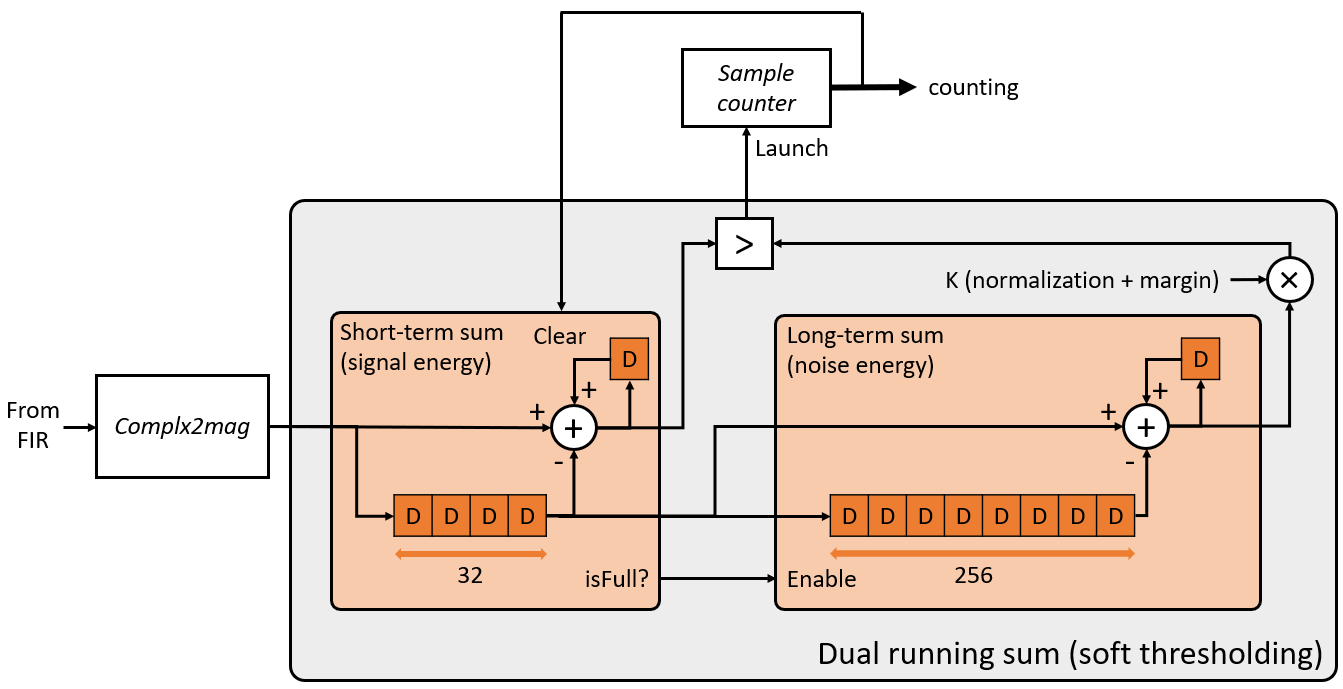
\includegraphics[width=\linewidth]{figures/dual_running_sum_block.png}
        \caption{Architecture of the dual running sum}
        \label{fig:dual_runnign_sum}
    \end{figure}

    The overall architecture of the dual running sum is shown in Fig. \ref{fig:dual_runnign_sum}. When packet samples arrive, possibly with  higher energy than the noise, they first enter the first delay line. Its accumulator value therefore increases and might at one point exceed the accumulator value of the second line, which contains only noise sample. At this point, a packet is considered present and a launch signal is triggered.

    To be noted, when a packet is detected and the counter (next block) is enabled, we clear the short-term sum and disable the long-term one, to avoid any retriggering or corruption of our noise evaluation by packet samples.


    \item \textbf{Counter :} This block receives the launch signal of the previous one. This counter block is used to count the samples when the threshold has been reached and avoid triggering a start flag multiple times inside a single packet. A \texttt{launch} signal starts the counter, it stops only after reaching its maximum value. During the sequence a \texttt{running} signal indicates the state of the counter. This signal is used to clear the short-term sum of the dual running sum.

    \item \textbf{Flag addition :} A multiplexer is used at the end to set a sample to a flag, here $I=$\texttt{0x7FF} and $Q=$\texttt{0x7FF}  when the launch signal is triggered.

\end{enumerate}


\begin{figure}[h]
    \centering
    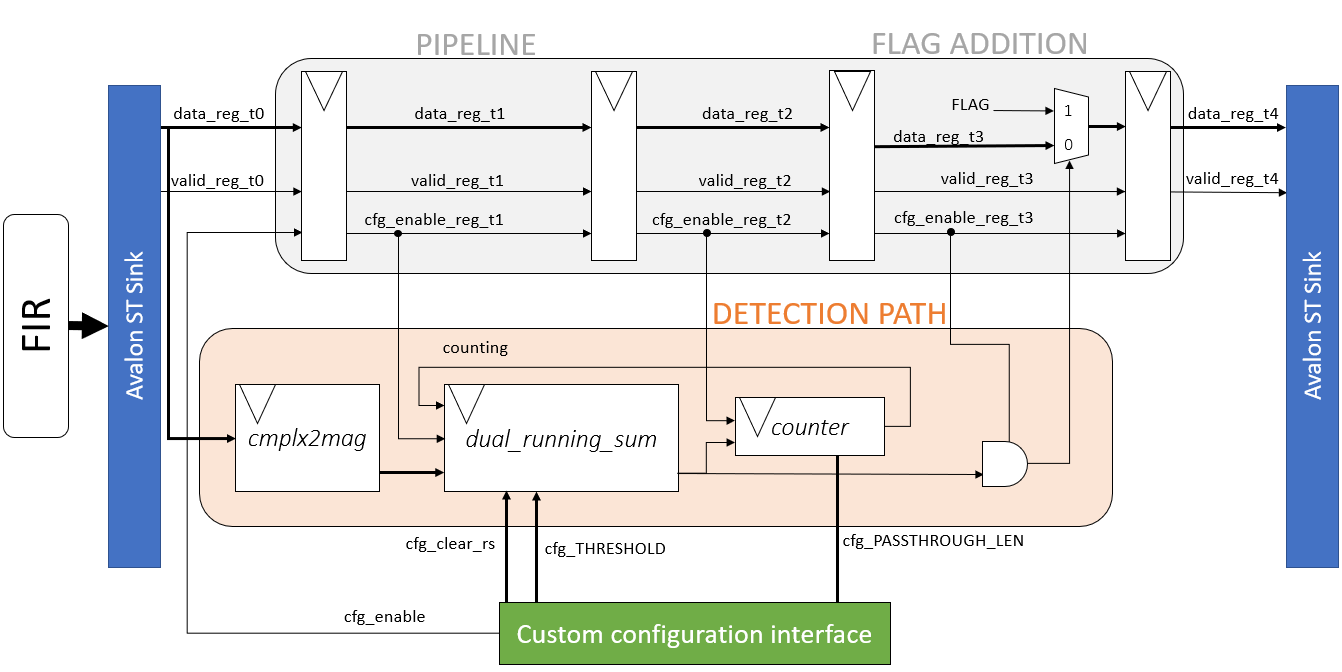
\includegraphics[width=\linewidth]{figures/packet_presence_detection.png}
    \caption{Hardware packet presence detector schematic}
    \label{fig:pd_schematic}
\end{figure}

In order to reduce the length of the critical path between registers, we use a paradigm called \textit{pipelining}. In short, we divide the operations of the PPD into several stages with similar length. As the critical path in this configuration is much shorter, it allows to operate the circuit at a higher frequency. In return, the additional registers add area and energy consumption to the design. It also requires to forward control signals in the pipeline and it can add complexity (see \textit{Control Path} in Figure \ref{fig:pd_schematic}). You will learn the concept of pipelining in details when studying the \textit{pipelined processor} in the course of \texttt{LELEC2531}.

Try to understand the SystemVerilog implementation of those blocks with respect to their theoretical behavior. Pay particular attention to the bus width of intermediate signals, they are computed in order to systematically avoid any overflow of intermediate values!


\subsection{Modification and simulation of the PPD}


We will first ask you to make some modifications to the dual running sum, more specifically to the comparison between the short- and long-term sum results. In order to make it adaptative from GNU Radio, we will use the \texttt{cfg\_THRESHOLD} signal of the packet presence detection module to multiply the result of the long-term sum before comparing it to the short-term sum result. This allows to be more selective regarding the signal-to-noise ratio required to detect the packet. Increasing its value will limit the risk of false alarm due to noise but make your system less sensitive. In short, with this parameter set to 10, the PPD would require a signal magnitude 10 times higher than the noise one to trigger a detection. However, we should also normalize the short-term and long-term result with respect to the delay line length, the second one being here eight times longer than the first. Overall, we ask you to implement the multiplication shown in Figure \ref{fig:dual_runnign_sum}. In the SystemVerilog code, go to the line 199. We ask you to implement both the normalization, i.e. division by eight, and the multiplication operation on the same line. Note that the \texttt{cfg\_THRESHOLD} signal is connected to the \texttt{K} input of the dual running sum module.


\begin{bclogo}[couleur = gray!20, arrondi = 0.2, logo=\bcquestion]{Division by eight}
    \begin{itemize}
        \item Performing multiplications and divisions is much more complex than simple additions. However, when performing operations with values that are power-of-two, things always seem easier. What would be an efficient way to perform the division by eight?
        \item The order in which the two operations are performed, here the multiplication by K and division by eight would normally have no importance. Is it the case here? Which operation should be performed first and why?
    \end{itemize}
\end{bclogo}

Once you have implemented this function, we should now test the PPD. We have developped a testbench for you, and we will use ModelSim to verify the PPD behavior before deploying it into the complete system. A few python scripts located at \texttt{ip/packet\_presence\_detection/testbench/python} allow you to generate input vectors for the PPD and compare the testbench output with an expected result obtained with python:

\begin{enumerate}
    \item \texttt{1\_input\_gen.py} : generates input vectors and export them as input vector of the PPD HDL implementation.

    \item To generate the testbench, we will use the \textit{Platform Designer}. It allows the interconnection of multiple blocks of a digital design with a more intuitive user interface. Open the \textit{Platform Design} using the shortcut highlighted in Figure \ref{fig:quartus_platform_designer}. Open the \texttt{packet\_presence\_detection\_tb\_gen}, and go in \textit{Generate} in the upper left corner, then \textit{Generate Testbench System}. Change the path to \texttt{LimeSDR-Mini\_lms7\_lelec210x/ip/packet\_presence\_detection/} and click on \textit{Generate}. To execute the testbench, open ModelSim and change the working directory to\\ \texttt{ip/packet\_presence\_detection/testbench}. Then run \texttt{do run\_sim.tcl} in order to compile and launch the simulation.

\begin{figure}[H]
    \centering
    \includegraphics[scale=0.7]{figures/quartus_toolbar.PNG}
    \caption{Toolbar of Quartus. The Platform Designer shortcut is highlighted in yellow.}
    \label{fig:quartus_platform_designer}
\end{figure}

    \item \texttt{2\_compare} : when the SystemVerilog testbench has been executed, compares the input data samples to the output of the PPD, plotting them. If it works as expected, the only difference should be the addition of the flag.
\end{enumerate}

Once you have analysed the results, we will propagate the changes you made to the complete system that will be flashed on the FPGA. Remember we only modified the IP, we now need to propagate those changes to the actual design. In the \textit{Platform Designer}, open the \texttt{lms\_dsp.qsys} design. Nothing has to be done except clicking \textit{"Generate HDL ..."} on the bottom right of the window and update the path to
\texttt{LimeSDR-Mini\_lms7\_lelec210x/lms\_dsp/} if it is not made automatically. Then press on \textit{"Generate"}. The changes you made locally to the PPD have now been propagated. In the Platform Designer, you can quickly observe the structure of the \textit{lms\_dsp} block, with the FIR, the packet presence detection and the different Avalon Streaming Interface.

You can now compile your design and observe the resource and timing report. Be careful when launching a compilation in Quartus, a window may ask you to update the project revision. Answer \textit{"NO"}.

\begin{bclogo}[couleur = gray!20, arrondi = 0.2, logo=\bcattention]{MAX 10 Device Support might not be installed}
    The support for the FPGA device we use might not be installed in the Quartus you have, which will lead to errors in the compilation. The installation instructions are provided in the wiki of the course.

\end{bclogo}

\subsection{Timing and ressource analysis}

As you have seen in course, an important aspect of digital design is to ensure that your design meet both the resource and timing requirements. Indeed, long combinatorial logic path can lead to setup or hold constraints violations. Now that the design has been compiled, you can check the compilation report using the shortcut highlighted in Figure \ref{fig:compilation_report_button}.

\begin{figure}[h]
    \centering
    \includegraphics[width=\linewidth]{figures/Compilation_report_button.PNG}
    \caption{Toolbar of Quartus. The Compilation Report shortcut is highlighted in red.}
    \label{fig:compilation_report_button}
\end{figure}


In the \textit{"Flow Summary"} tab, the resource utilisation is reported. Observe for instance the number of embedded multipliers that are employed. Moreover, in the \textit{"Analysis \& Synthesis/Timing Analyzer"} tab, you can see the results for the different corners, constraints violations being highlighted in red. Try to identify the faulty clock involved. In the different summary proposed, you can right click on a clock and select \textit{"Report Timing... (In Timing Analyzer UI)"}. In the opened window, just press \textit{"Report Timing"} at the bottom. Those steps are depicted in Figure \ref{fig:report_timing_analyzer}. You can now analyze the most critical path implying the selected clock, as well as the logic cells involved. Try to link the critical path to the RTL design. It should involve a signal starting in the dual running sum module. An easy fix is here to add a register in the path to break in two. This will delay the launch signal by one clock cycle, which is not problematic.

\begin{figure}[h]
    \centering
    \includegraphics[width=\linewidth]{figures/Report_Timing_Analyzer.png}
    \caption{Steps to analyze the most critical path on a given clock.}
    \label{fig:report_timing_analyzer}
\end{figure}

Moreover, we prevented \textbf{register retiming} which allows the synthesis tool to balance the combinatorial logic across registers when it does not affect the system behaviour. This helps on meeting the timing requirements by offloading parts of long combinatorial path. To enable this setting, go in \textit{"Assignments/Settings/Compiler Settings"} on Quartus and uncheck the \textit{"Prevent register retiming"} box.

Before relaunching a compilation, ask for an assistant to check your modifications, to avoid wasting precious synthesis time. Done? Now relaunch a compilation and analyze the results. Again, if a window asks you to update the project revision, answer \textit{"NO"}. Is there still a timing constraint violation? Can you still link the most critical path to the HDL design?

To analyse the ressource used by the design, you can look at the \textit{Project Navigator} tab in \textit{Hierarchy}. More than navigating through the design, you can also look at the ressource used by each module. Analyse the resource usage of the PPD, more specifically the memory bits and the DSP.
\begin{comment}
\subsection{From Euclidean norm to Absolute-value norm}

In order to meet the timing requirements, another solution is to use a less complex estimation of the IQ samples magnitude. We are thus going to use a very simple and accurate algorithm that does not have the burden of implementing the complex logic of \textit{integer multiplication}. The estimate for the first quadrant of the trigonometric circle is drawn on Figure \ref{fig:cmplx2mag}. We ask you to implement it in System Verilog, the mathematical formula being provided to you in Equation \ref{eq:1norm}\footnote{Further information can be found online: \url{https://en.wikipedia.org/wiki/Alpha_max_plus_beta_min_algorithm} and \url{http://dspguru.com/dsp/tricks/magnitude-estimator/}.}. Your modification of the \texttt{cmplx2mag} module must be done in the \texttt{USER CODE} parts, which goes from line 45 to 52 and on line 210. As we were performing two multiplications and one addition in the previous algorithm ($I^2+Q^2$), the data bus at the output of the \textit{cmplx2mag} module was specified as twice the input data bit width (due to multiplication) plus one (due to the addition). This is specified on line 210, do not forget to adapt it for the new algorithm. In the next step, you are going to make a behavioral simulation of you implementation to validate it.

\begin{equation}
    |z| = \frac{min(|I|,|Q|)}{4} + max(|I|,|Q|)
    \label{eq:1norm}
\end{equation}

\begin{figure}[h]
    \centering
    \includegraphics[width=0.45\linewidth]{figures/trigo.png}
    \includegraphics[width=0.45\linewidth]{figures/angle.png}
    \caption{Complex Magnitude Estimator output in x-y coordinates (left) or polar coordinates (right) for input points of the trigonometric circle.}
    \label{fig:cmplx2mag}
\end{figure}


Now that you have a functional design for the preamble detector with the Absolute-value norm, we can perform a synthesis of the complete design. Do not forget to propagate your change by regenerating the HDL via the Platform Designer. Observe the resource usage and the timing report, is there still a timing constraint violation?

\end{comment}

\section{Practical part}
%
Similarly \emph{hands\_on\_mcu.pdf}, you can run the code by:
\begin{itemize}
	\item Flashing the MCU with the code by clicking on the green run button.
	\item Launching the script reading the content of the uart printed by the MCU with \texttt{python uart-rader.py -p PORTNAME}. 
\end{itemize}
If your python script runs, pressing the \textcolor{blue}{User blue button} on the Nucleo board should launch an audio acquisition with the microphone. A figure should open, showing the acquired melspectrogram. To stop your script, click on \texttt{CLTR+C} in the command prompt then press the \textcolor{blue}{User blue button} again.  Remember how to switch to an audio acquisition with the jack cable by changing the \texttt{SEL\_SOUND} pin connection on the Nucleo board as explained in \emph{hands\_on\_audio\_acquisition.pdf}. 
%
%%%%
\subsection{Embedded computations and complexities}
%
You are now ready to dive into a new embedded programming project. 
We restart from the end of \emph{hands\_on\_audio\_acquisition.pdf}, i.e. where you implemented the double buffering for sampling your signal with the ADC. What is new in this project is the content of the function called when you press the \textcolor{blue}{User blue button}: \\
%
\begin{lstlisting}
void HAL_GPIO_EXTI_Callback(uint16_t GPIO_Pin) {
	if ((GPIO_Pin == B1_Pin) & !bounce) {
		HAL_ADC_Start_DMA(&hadc1, (uint32_t *) ADCBuffer, 2 * SAMPLES_PER_MELVEC);
		HAL_TIM_Base_Start(&htim3);
		bounce = 1;
	}
}
\end{lstlisting}
%
Where you start the DMA each time the button is pressed. We also changed the content of \newline HAL$\_$ADC$\_$ConvCpltCallback for these two functions:
%
\begin{lstlisting}
void HAL_ADC_ConvHalfCpltCallback(ADC_HandleTypeDef *hadc) {
	Spectrogram_Format((q15_t *)ADCDblBuffer[0]);
	Spectrogram_Compute((q15_t *)ADCDblBuffer[0], mel_vectors[cur_melvec]);
	cur_melvec++;
	DEBUG_PRINT("Half DMA.\r\n");
}
\end{lstlisting}
\begin{lstlisting}
void HAL_ADC_ConvCpltCallback(ADC_HandleTypeDef *hadc) {
	Spectrogram_Format((q15_t *)ADCDblBuffer[1]);
	Spectrogram_Compute((q15_t *)ADCDblBuffer[1], mel_vectors[cur_melvec]);
	cur_melvec++;
	if (cur_melvec == N_MELVECS)
	{
		HAL_TIM_Base_Stop(&htim3);
		HAL_ADC_Stop_DMA(&hadc1);
		print_buffer(mel_vectors_flat, N_MELVECS * MELVEC_LENGTH);
		cur_melvec = 0;
	}
	bounce = 0;
	DEBUG_PRINT("All DMA.\r\n");
}
\end{lstlisting}
%
Which compute one feature vector each time the button is pressed. \\
You can find a new file \emph{spectrogram.c} which details exactly how we do the computations, which functions are used and why. We left lots of comments with some questions to ensure you follow it. Note you can vary the parameters in \emph{config.h}. \\
\\

\begin{bclogo}[couleur = gray!20, arrondi = 0.2, logo=\bcinfo]{Casting data}
%
In the step $3.2$ of \emph{spectrogram.c}, you will observe this line of code:
%
\begin{lstlisting}
buf[i] = (q15_t) (((q31_t) buf_fft[i] << 15) / ((q31_t) vmax));
\end{lstlisting}
%
In this line, the (q15$\_$t) and two (q31$\_$t) are called \textbf{casting}. This consists in telling your compiler the format you wish the following variable to be stored in. Here, buf$\_$fft[i] is in q15$\_$t format, and the $\ll 15$ shift all its bits to the left $15$ times. The casting is necessary to get a temporary q31$\_$t variable and avoid overflowing your q15$\_t$ one.
%
\end{bclogo}
%
\begin{bclogo}[couleur = gray!20, arrondi = 0.2, logo=\bcinfo]{Hardcoding data}
The content of \emph{spectrogram$\_$tables.h} and \emph{spectrogram.h} has been hardcoded using the files in \textbf{Python2C$\_$conversion}. These notebooks could be useful for you during the second semester if you want to apply your feature vector computations on a perfect signal, i.e. an audio signal from the Dataset which has directly been hardcoded in C. This is optional, but you can already take a look at how this is done.
\end{bclogo}
%
When you read and try to understand the code (remember this is equivalent to what you did during H1 in Python), \textbf{evaluate the theoretical complexity of the different functions involved} ($\mathcal O(n^2)$, $\mathcal O(\sin (n))$,\ldots), this will help you to identify the \emph{bottlenecks} (worst parts in a computational point of view). Each time you have a pipeline with different computations where the efficiency is critical, you should work on improving your bottlenecks. Confirm your evaluations of the computational complexities by \textbf{measuring the cycle counts of all intermediate computations in spectrogram.c} as explained in \emph{hands\_on\_authentication.pdf}.
Think about it and \textbf{discuss with the TA's your ideas to improve} what we propose. \\
\\
For now, the feature vector content is printed on the UART and displayed on the console (e.g. Putty). The function which reads the printed content (in \emph{hex}) is \textbf{uart$\_$reader.py}. It is fairly short. Understand what it does and add your functionalities from what you have done for the hands-on session on the classification aspects to \textbf{apply a classification on the feature vector}. \\
\\
%
\noindent To summarize, you have to:
\begin{enumerate}
    \item Be able to run and understand the provided code.
    \item Check the consistency between a melspectrogram obtained only in simulation (as in H1) and obtained through the jack cable. Except for a random scaling, they should be almost identical.
    \item Evaluate the theoretical complexities and measure the cycle counts of the operations made in \emph{spectrogram.c}.
    \item Modify \emph{uart$\_$reader.py} to test your trained classifier on the computed feature vector.
\end{enumerate}
%
%%%%
\subsection{Calibrated dataset}
%
You should have noticed that the performances of your trained classifier on audio signals acquired with the microphone are very poor. Indeed, there are many differences between a nice feature vector computation made from a registered audio file in Python and a real computation made from an acquired signal in fixed-point format in C.

To take these imperfections into account, you will create training data using your own device. It implicitely takes the acquisition non idealities into account, and gives you the possibility to truly augment the data increasining the distance between the sound source and microphone, or adding background sound by yourself.
%
\noindent To summarize, you have to:
\begin{enumerate}
    \item Modify \emph{uart\_reader.py} to save the computed feature vectors in your system and create a new dataset of feature vectors.
    \item Train a classifier on this new dataset.
\end{enumerate}


%%%%%%%%%%%%%%%%%%%%%%%%%%%%%
\section{Report R5}
%
The report R5 (due on \textbf{Dec 4, Monday 23.55 PM}) focuses on the characterization of the feature vector extraction and the associated classification model. We name \emph{H5a} the three Python notebooks related to the classification aspects and \emph{H5b} the instructions in this pdf related to acquisition and classification using the MCU. We expect you to:
%
\begin{itemize}
    \item (H5a) \textbf{Characterize a classification model of your choice on the provided audio dataset, provide chosen performance metrics and detail the validation method you used. Briefly justify your choices.}
    \begin{itemize}
        \item The classification model has to be different from the provided KNN such that you reproduce the analyzes given in hands\_on\_classif2\_audio.ipynb (have a look here :\\ \url{https://scikit-learn.org/stable/supervised\_learning.html#supervised-learning}).
        \item The metrics can be the accuracy and confusion matrix, but can also be other ones as long as you justify their relevance.
        \item The validation method is the way you split the dataset in learning, validation and testing sets.
        \item You must specify if you considered normalization of the feature vectors and if you introduced data augmentation (if so, which ones and why?)
    \end{itemize}
    In short, we ask a paragraph explaining why you chose your model, the used metrics, and validation methods, then one figure with its performances on the testing set. We also ask a figure showing the influence of potential hyperparameters of your model and a discussion on what you observe from it. You won't be evaluated on the performances of the chosen classification model, we are only interested in the quality of your analysis.
    \item (H5b) \textbf{Provide a table giving the computational complexities and cycle counts of the feature extraction pipeline on the MCU} written in \emph{spectrogram.c}. Which transformation requires the most computations? \\
The feature vector computation simply consists in a chain of well-known mathematical operations with given computational complexity. We ask you to compute the overall complexity when putting it all together.
\item (H5a+H5b) \textbf{Observe and discuss qualitatively the difference observed between melspectrograms:} 
\begin{enumerate}
    \item of the original dataset
    \item acquired via a jack cable on the MCU
    \item acquired via the microphone on the MCU.
   \end{enumerate}
   To help this comparison, we advise you to show the whole melspectrogram on the 5s-long audio signal in Python, and to identify in this whole melspectrogram what is the subpart that is the most related to your acquired melspectrogram with the Nucleo board.
   %
     Use \textbf{a few} representative samples of the dataset to conduct your experiments.
       We ask, for each sample, a (1,3) subplot showing the melspectrograms for cases 1,2,3 from left to right. Please make it clear with titles or captions in your figures.
    \item (H5a+H5b) \textbf{Explain how you created a new dataset of acquired feature vectors.} What data augmentation techniques did you consider in this calibrated dataset? Train a classification model on this dataset. 
    \item (H5a+H5b) \textbf{Demonstrate the performance of your classification model on feature vectors acquired with the microphone on the MCU.}
    Make this evaluation with a few samples of your choice. We ask at least 3 sounds from each of the 5 classes (crackling fire, chirping bird, chainsaw, helicopter and handsaw) in order to see something.
    \item (H5a+H5b) \textbf{Discuss the effect of exploiting memory effect for your classification model in the context of environmental monitoring. Why will it be useful in practice? Implement a combination of consecutive probability vectors.} We ask you to exploit the memory effect of consecutive feature vectors coming from the same class. You are free to choose any combination of these feature vectors discussed in \emph{hands\_on\_classif3\_trust\_and\_memory.ipynb}. We ask at least one sound from 2 out of the 5 classes (crackling fire, chirping bird, chainsaw, helicopter and handsaw).
\end{itemize}

\subsection{SystemVerilog parameters}
When instantiating the IP in the subsystem, you are allowed to define the values of a few \textit{SystemVerilog parameters} for the top-level module of the preamble detector, as shown in Figure \ref{fig:pd_hard_param}. Those parameters described in the Table \ref{table:pd_hard_param}.

\begin{figure}[!h]
    \centering
    \includegraphics[width=\linewidth]{figures/preamble_detect_qsys_config.PNG}
    \caption{SystemVerilog parameters of the preamble detector in QSYS.}
    \label{fig:pd_hard_param}
\end{figure}

\begin{table}[!h]
\centering
\begin{tabular}{|p{0.36\linewidth}|p{0.48\linewidth}|p{0.08\linewidth}|}
\hline
Parameter & Description & Default value \\
\hline
\textsc{DATA\_WIDTH} & Bit width of the samples & 12 \\
\hline
\textsc{FILTER\_LEN\_WIDTH} & Bit width of the configurable moving average filter length & 6 \\
\hline
\textsc{PASSTHROUGH\_LEN\_WIDTH} & Bit width of the configurable number of samples to pass-through once the threshold is reached & 16 \\
\hline
\end{tabular}
\caption{SystemVerilog parameters of the \texttt{preamble\_detector} IP}
\label{table:pd_hard_param}
\end{table}

\subsection{Configuration signals}
\begin{sloppypar}
Additionally, there are several configuration signals that can be changed during operation from GNU Radio for better flexibility. Those configuration signals are listed in Table \ref{table:pd_soft_param}, you can trace them in the VHDL code, they are coming from the \texttt{fpgacfg} module defined in \texttt{LimeSDR-Mini\_lms7\_lelec210x/src/spi/fpgacfg.vhd}and located in the design hierarchy at \texttt{lms7\_trx\_top/inst0\_nios\_cpu/cfg\_top\_inst1/fpgacfg\_inst0}, as shown in Figure \ref{fig:design_hier_fpgacfg}.
\end{sloppypar}

This module contains a RAM with 16-bit words that retains the configuration of various elements of the FPGA. We used available addresses to put our custom configuration, the address map is written in the repo README. There are default values assigned at reset for the memory bits (Figure \ref{fig:design_hier_fpgacfg}) but they can be changed with a write operation.

\begin{table}[!h]
\centering
\begin{tabular}{|p{0.22\linewidth}|p{0.25\linewidth}|p{0.34\linewidth}|p{0.08\linewidth}|}
\hline
Configuration signal & Description & Allowed values\\
\hline
\texttt{cfg\_enable} & Enable or disable the preamble detector. When disabled, the samples are always passing through. & $\left\{0,1\right\}$ \\
\hline
\texttt{cfg\_FILTER\_LEN} & Size of the moving average filter. & $\left[1,2^{\textsc{FILTER\_LEN\_WIDTH}}-1\right]$ \\
\hline
\texttt{cfg\_PASSTHROUGH\_LEN} & Number of samples to pass-through once the threshold is reached. & $\left[1,2^{\textsc{PASSTHROUGH\_LEN\_WIDTH}}-1\right]$ \\
\hline
\texttt{cfg\_THRESHOLD} & Value to be compared with the moving average filter output. & $\left[1,2^{32}-1\right]$ \\
\hline
\end{tabular}
\caption{Configuration signals \texttt{preamble\_detector} IP}
\label{table:pd_soft_param}
\end{table}

\begin{figure}[!h]
    \centering
    \includegraphics[width=0.3\linewidth]{figures/design_hierarchy_fpgacfg.PNG}
    \includegraphics[width=0.6\linewidth]{figures/design_hierarchy_fpgacfg_both.PNG}
    \caption{Configuration signal location in the design hierarchy (left). Assignment and reset values for the DSP configuration signals (right).}
    \label{fig:design_hier_fpgacfg}
\end{figure}

\subsubsection{Read/write operations of the configuration signals from GNU Radio}
The GNU Radio block of the LimeSDR-Mini uses a C++ library called \textit{LimeSuite} in order to write data to the FPGA configuration memory. In the following paragraph, the configuration flow inside LimeSuite and the hardware is briefly described.

\begin{sloppypar}
\paragraph{gr-limesdr GUI interface}
In our custom version of the limeSDR GNU Radio block, we added fields to configure the hardware preamble detector. To do so, we modified the file \texttt{gr-limesdr/grc/limesdr\_fpga\_source.block.yml} and added a GUI callback function named \texttt{set\_dspcfg\_preamble}. This function is in turn defined in \texttt{gr-limesdr/lib/source\_impl.cc} and \texttt{gr-limesdr/lib/device\_handler.cc}. Please take a look at the end of \texttt{device\_handler.cc} and understand the functions we added. At the core of all of them, we use \texttt{modify\_spi\_reg\_bits}, shown in Figure \ref{fig:modify_spi_reg_bits}, that uses LimeSuite \texttt{LMS\_WriteFPGAReg} function. Pay attention to the arguments and try to make the link with the configuration memory of the FPGA, the input structures are defined in \texttt{gr-limesdr/lib/fpga\_register\_map.h}.
\end{sloppypar}

\begin{figure}[!h]
    \centering
    \includegraphics[width=\linewidth]{figures/grlimesdr_write_fpgacfg.PNG}
    \caption{Software interface between GNU Radio and LimeSuite.}
    \label{fig:modify_spi_reg_bits}
\end{figure}

\paragraph{NIOS Interface}
When calling \texttt{LMS\_WriteFPGAReg}, the functions wrap the address and value of the register we wish to configure inside a packet that is transmitted through USB. The complete callstack inside the library is described in the repo README. The USB interface is connected to an FTDI Chip which is in turn interfaced with the FPGA, as shown in Figure \ref{fig:limesdr_mini_schematic}.

Inside the FPGA, we have:
\begin{enumerate}
    \item An FTDI arbitrer that decodes a first part of the packet header to forward it through a configuration FIFO (\texttt{EP02\_fifo}) towards the NIOS subsystem. This arbitration is necessary as we have two other FIFOs coming from the NIOS subsystem and the RX data path (\texttt{EP83\_fifo} and \texttt{EP82\_fifo} respectively).
    \item A NIOS Softcore processor instantiated inside the FPGA reads the FIFO and decodes the second part of the packet header, it then forwards the packet data to through an SPI Master.
    \item An SPI Slave is connected with the configuration memory and writes the received data at the correct address.
\end{enumerate}

\begin{bclogo}[couleur = gray!20, arrondi = 0.2, logo=\bcinfo]{Additional resources}
To help you understand this complex path, we provided you with resources you can find on moodle or \texttt{LimeSDR-Mini\_lms7\_lelec210x/doc/} folder. The file \texttt{FPGA\_config\_path.pdf} with annotations referring to the above paragraph should be helpful, several elements have been hidden to ease the reading. You can also use freely the RTL viewer to skim through the design hierarchy graphically instead of opening files, see Figure \ref{fig:rtl_viewer} for further details.
\end{bclogo}

\begin{figure}[!h]
    \centering
    \includegraphics[width=0.7\linewidth]{figures/limesdrmini_schematic.png}
    \caption{Location of the different chips on the LimeSDR-Mini board.}
    \label{fig:limesdr_mini_schematic}
\end{figure}

\begin{figure}[!h]
    \centering
    \includegraphics[width=0.7\linewidth]{figures/rtl_viewer.png}
    \caption{In order to use the RTL viewer, first elaborate the design (1) then right click on the design element you want view (2).}
    \label{fig:rtl_viewer}
\end{figure}




\end{document}
%%%%%%%%%%%%%%%%%%%%%%%%%%%%%%%%%%%%%%%%%%%%%%%%%%%%%%%%%%%%%%%%%%%%%%%%%%%%
